%************************************************
\chapter{Domain Name Service and Service Discovery}\label{ch:dns}
%************************************************
\textit{Topic 5: Write a brief introduction to Domain Name Service and Service Discovery and use these descriptions to put perspective on your report. The perspectives should include:
- How may Domain Name Services be beneficial in cluster and cloud computing?
- How may Service Discovery be beneficial in cluster and cloud computing?}

The Domain Name System (DNS) is a kind of translation system that allows humans to search the internet using language we are comfortable with. So in other word DNS allows you to type names into the Web browser like www.youtube.com and automatically find that address on the Internet, instead of type the IP-address of the web site.

The DNS organizes its servers into a hierarchy figure \ref{fig:DNShierarchy} shows the hierarchy. For the Internet, so-called root name servers reside at the top of the DNS hierarchy. The root servers are responsible for holding information about all the top level domains, it is the starting point for every name lookup operation. Top level domains is divided into two groups:

\begin{itemize}
\item \textbf{Generic Top Level Domains (gTLD) .com, .edu, .net, .org, .mil etc.}
\item \textbf{ Country Code Top Level Domain (ccTLD) e.g. .us, .ca, .tv , .uk etc.}
\end{itemize}
Each ccTLD identifies a particular country and is two letters long.  At the domain level or user DNS you have the resource you are looking for.\begin{figure}[bth]
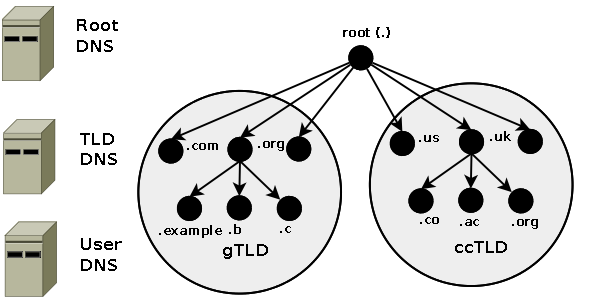
\includegraphics[width=1\linewidth]{gfx/DNShierarchy}
\caption[routingtable]{Routing table for Pastry} \label{fig:DNShierarchy}
\end{figure}
\\
\textbf{Recursive Query Vs Iterative Query in DNS}

A recursive query is a kind of query, in which the DNS server, who received the query, will do the entire job fetching the answer, and giving it back to client. If DNS server is not able to resolve the requested query then it forwards the query to another DNS server until it gets an answer or the query fails.
In an iterative query, the name server, will not go and fetch the complete answer for the query. If the queried DNS server does not have an exact match for the queried name, the best possible information it can return is a referral, which might have the answer. The DNS client can then query the DNS server for which it obtained a referral.
\\\\
\textbf{Cached queries}

DNS caching allows any DNS server or client to locally store the DNS records and re-use them in the future. The Ip and domain is stored in local cache called stub-resolver for a period. By that, we obtain a reduced network usage, higher efficiency, lower number of packets and thereby a lower latency. 
\\\\
\textbf{How may Domain Name Services be beneficial in cluster and cloud computing?}

Ved at have redundant DNS, hvis en af dem skulle gaa ned.
To create additional resilience each root-server typically has multiple instances (copies) spread throughout the world. Each instance has the same IP address but data is sent to the closest instance using a process called anycasting.
